\section{Metodologia}
\label{Metodologia}

% %Aqui precisamos colocar um diagrama/arquitetura mostrando o fluxo%
% A metodologia adotada neste trabalho compreende o desenvolvimento integrado de um sistema embarcado para o monitoramento contínuo de sinais vitais e a construção de modelos de aprendizado de máquina para a predição antecipada do do NEWS2. O sistema é estruturado em três camadas: (i) a camada de aquisição, composta pelos sensores responsáveis pela coleta dos parâmetros fisiológicos do paciente; (ii) a camada de processamento embarcado, encarregada do pré-processamento dos sinais, do cálculo NEWS2 atual e da execução do modelo preditivo; e (iii) a camada de saída, responsável pela exibição dos escores e pela sinalização de alertas à equipe assistencial. Para o desenvolvimento e a validação dos modelos preditivos, são utilizados dados clínicos provenientes de bases públicas de pacientes hospitalizados \cite{REYNA}, sendo treinados e comparados três algoritmos com vieses indutivos distintos, de modo a identificar a abordagem mais adequada ao contexto de execução embarcada. A Figura 1 ilustra a arquitetura geral do sistema proposto. 

% %acho que é essencial colocarmos a arquitetura/figura do sistema%

Esta seção apresenta primeiramente os materiais escolhidos para o desenvolvimento do dispositivo, bem como a justificativa para o seu uso. Em seguida, para a descrição do método, adotou-se uma abordagem dividida em etapas direcionadas ao hardware e etapas direcionadas ao software. As etapas voltadas ao hardware abrangem a montagem física do dispositivo e a integração entre a placa de processamento, os sensores e os periféricos. Já as etapas voltadas ao software contemplam a configuração do sistema operacional embarcado, a comunicação com os sensores, o processamento dos sinais fisiológicos, o cálculo do escore NEWS2 e o desenvolvimento do modelo preditivo de deterioração clínica.

\subsection{Materiais}

% Plataforma
A plataforma de processamento é responsável pela execução do sistema 
operacional embarcado, pela aquisição dos sinais fisiológicos, pelo 
processamento dos dados coletados, pelo cálculo do escore NEWS2 e pela 
execução dos modelos de aprendizado de máquina empregados na predição de 
deterioração clínica. Com isso, foi escolhida a Raspberry Pi 3B+, uma vez que possui ampla documentação para o Buildroot, comunidade ativa, memória RAM de 1 GB, arquitetura 
quad-core de 64 bits a 1,4 GHz e disponibilidade nativa de interfaces
I\textsuperscript{2}C, SPI, HDMI e DSI.

% Sensoriamento
A partir dessa plataforma, a extração dos parâmetros do NEWS2 é realizada por dois sensores. O sensor PPG MAX30102 reúne LEDs vermelho e infravermelho, que viabilizam a extração da SpO\textsubscript{2}, em um encapsulamento compacto, com ADC de 18 bits e baixo custo. Sua interface I\textsuperscript{2}C é nativamente suportada pelo \textit{kernel} Linux, dispensando \textit{frameworks} de terceiros e viabilizando a implementação de um \textit{driver} dedicado em C++. Já o sensor de temperatura DS18B20 oferece resolução configurável de até 12 bits, correspondente a incrementos de 0,0625°C, e precisão de ±0,5°C na faixa de operação corporal. Sua interface digital 1-Wire, também suportada nativamente pelo \textit{kernel}, dispensa ADC externo e permite a leitura da temperatura diretamente via sistema de arquivos, simplificando a integração ao sistema embarcado.

% O MAX30102 se destaca entre os analisados por reunir LEDs vermelho e infravermelho - que viabilizam a extração da SpO\textsubscript{2} - em um encapsulamento compacto, ADC de 18 bits e baixo custo. Além disso, sua interface I\textsuperscript{2}C é nativamente suportada pelo kernel Linux, dispensando \textit{frameworks} de terceiros e viabilizando a implementação de um \textit{driver} dedicado em C++.

% O DS18B20 se destaca entre os analisados por apresentar resolução configurável de até 12 bits, correspondendo a incrementos de 0,0625°C, e precisão de ±0,5°C na faixa de operação corporal. Sua interface digital 1-Wire, nativamente suportada pelo kernel Linux por meio do driver \texttt{w1-therm}, dispensa ADC externo e permite a leitura da temperatura diretamente via sistema de arquivos, simplificando a integração ao sistema embarcado.

% Perifericos
Para o \textit{feedback} visual, optou-se pelo \textit{display} Waveshare de 7 polegadas, cujo tamanho de tela garante alta legibilidade à beira do leito, com compatibilidade direta via HDMI e suporte a toque capacitivo. Complementando o sistema de alertas, o \textit{buzzer} piezoelétrico emite sinais sonoros quando o escore NEWS2 atinge limiares de risco elevado, enquanto o LED RGB reproduz a codificação de cores do protocolo de forma perceptível à distância. Ambos operam via GPIO, sem circuitos de controle adicionais além de resistores limitadores de corrente.

% Como forma de dar \textit{feedback} imediato foi escolhido o \textit{display} Waveshare de 7 polegadas, uma vez que o seu tamanho de tela garante alta legibilidade e usabilidade à beira do leito, e possui compatibilidade direta via interface HDMI com a placa de processamento escolhida e ao suporte a toque capacitivo, que possibilita uma interação mais responsiva com a interface gráfica.

% O buzzer piezoelétrico e o LED RGB complementam o sistema de alertas de forma redundante e de baixo custo. O buzzer emite sinais sonoros quando o escore NEWS2 atinge limiares de risco elevado, garantindo que a equipe de saúde seja notificada mesmo sem visualizar o \textit{display}. O LED RGB, por sua vez, reproduz a codificação de cores do protocolo NEWS2 de forma sintética e imediatamente perceptível à distância, dispensando a leitura ativa do \textit{display} em situações de triagem rápida. Ambos os componentes operam via GPIO, sem necessidade de circuitos de controle adicionais além de resistores limitadores de corrente.

% Alimentação
Quanto à alimentação, optou-se por uma arquitetura conectada diretamente à rede elétrica, o que elimina limitações de autonomia energética e reduz a complexidade do projeto ao dispensar circuitos de gerenciamento de bateria. Para o protótipo, previu-se uma fonte chaveada AC-DC de 5 V, dimensionada para o consumo agregado do sistema e distribuída por um barramento que alimenta em paralelo a plataforma de processamento, o \textit{display} e os demais componentes. A adoção de uma fonte comercial simplifica a implementação do \textit{hardware} e contribui para a segurança operacional, alinhando-se às boas práticas de segurança elétrica para equipamentos eletromédicos estabelecidas pela norma IEC 60601-1 da \textit{International Electrotechnical Commission} (IEC) \citeonline{iec60601}.

% Diante desses requisitos, optou-se por uma arquitetura alimentada diretamente pela rede elétrica. Essa abordagem elimina limitações relacionadas à autonomia energética e reduz a complexidade do projeto ao dispensar circuitos dedicados ao carregamento e gerenciamento de baterias. Além disso, permite maior previsibilidade operacional e simplifica a manutenção do dispositivo.

% Para o protótipo, prevê-se a utilização de uma fonte chaveada AC-DC de 5 V e 3 A, responsável por alimentar a plataforma de processamento, os sensores, o display e os demais periféricos do sistema. A adoção de uma fonte comercial simplifica a implementação do hardware e contribui para a segurança operacional do equipamento, estando alinhada às boas práticas de segurança elétrica aplicadas a equipamentos eletromédicos, conforme estabelecido pela norma IEC 60601-1 da \textit{International Electrotechnical Commission} (IEC) \citeonline{iec60601}.

% Elementos mecanicos
Para a modelagem tridimensional da \textit{case} do dispositivo, utilizou-se o \textit{software} Autodesk Fusion, que dispõe de ferramenta CAD (do inglês \textit{computer-aided design}) com recursos de modelagem paramétrica e licenciamento gratuito para fins educacionais. A fabricação do invólucro foi realizada por manufatura aditiva pelo processo de Modelagem por Deposição Fundida (FDM, do inglês \textit{Fused Deposition Modeling}), em razão de seu baixo custo e facilidade de prototipagem, características que favorecem o desenvolvimento iterativo.

Quanto aos materiais, o Ácido Polilático (PLA, do inglês \textit{Polylactic Acid}) foi adotado nas iterações iniciais, em razão de sua facilidade de impressão e baixo custo, enquanto a versão final empregou o Polietileno Tereftalato Glicol (PETG, do inglês \textit{Polyethylene Terephthalate Glycol}), justificado por sua maior resistência térmica e tolerância à limpeza com álcool isopropílico, que é procedimento de higienização padrão em ambientes hospitalares.

% A modelagem tridimensional da \textit{case} do dispositivo foi utilizado o software Autodesk Fusion, o qual possui a ferramenta de projeto assistido por computador (CAD, do inglês \textit{computer-aided design}, que oferece recursos de modelagem paramétrica, colaboração em nuvem e licenciamento gratuito para fins educacionais e de desenvolvimento. Para a fabricação do invólucro do protótipo foi adotada a manufatura aditiva pelo processo de Modelagem por Deposição Fundida (FDM, do inglês \textit{Fused Deposition Modeling}) devido ao seu baixo custo de implementação, rapidez na produção de peças e facilidade de prototipagem, características que favorecem o desenvolvimento iterativo do produto.

% Para os materiais termoplásticos, foram utilizados dois materiais para etapas distintas do desenvolvimento. O Ácido Polilático (PLA, do inglês \textit{Polylactic Acid}) foi utilizado nas iterações iniciais do invólucro, em razão de sua facilidade de impressão, boa estabilidade dimensional e baixo custo.

% Para a versão final do protótipo, foi adotado o Polietileno Tereftalato Glicol (PETG, do inglês \textit{Polyethylene Terephthalate Glycol}). Essa é justificada por duas propriedades críticas para o contexto de aplicação do dispositivo: maior resistência térmica em relação ao PLA e tolerância à limpeza com álcool isopropílico, procedimento de higienização padrão em ambientes hospitalares e clínicos.


% Ferramentas de software
No âmbito do \textit{software}, o sistema embarcado, responsável pela comunicação com os sensores, pelo processamento dos sinais e pelo cálculo do NEWS2, foi desenvolvido em C++, escolhido por seu desempenho e controle fino sobre memória, determinantes em ambientes com recursos computacionais limitados \cite{knuttila2012functional}. O Buildroot foi selecionado como \textit{toolchain} de \textit{cross-compilação} para a construção de um sistema operacional personalizável baseado em Linux, em razão do desempenho demonstrado em trabalhos correlatos \cite{ozturk2023}.

Para os algoritmos de aprendizado de máquina, adotou-se a linguagem Python, consolidada nesse domínio por seu ecossistema robusto de bibliotecas especializadas e por favorecer a prototipagem rápida. Por fim, a interface gráfica embarcada foi desenvolvida com o \textit{framework} Qt, mantendo o C++ já adotado no restante do sistema embarcado, combinação madura e amplamente utilizada em sistemas embarcados \cite{qtAbout}.

% O Buildroot foi selecionado como toolchain de cross-compilação para o desenvolvimento de um sistema operacional personalizável baseado em Linux, devido ao desempenho demonstrado em trabalhos correlatos, como o de \citeonline{ozturk2023}. Para viabilizar o projeto de uma Placa de Circuito Impresso (PCB, do inglês \textit{Printed Circuit Board}), foi selecionado o Autodesk Fusion, uma vez que possui a ferramenta de Automação de Projetos Eletrônicos (EDA, do inglês \textit{Electronic Design Automation}), além de possuir uma curva de aprendizado rápida, interface intuitiva, licenciamento gratuito e um desenvolvimento colaborativo em nuvem.

% Para o desenvolvimento dos algoritmos de ML, foi adotada a linguagem de programação Python por ser amplamente consolidada nesse domínio por dispor de um ecossistema robusto de bibliotecas especializadas, que oferecem implementações otimizadas de modelos, pipelines de treinamento e ferramentas de avaliação. Ademais, a sintaxe simples e expressiva do Python favorece a prototipagem rápida e a legibilidade do código, aspectos relevantes em projetos de pesquisa que demandam iterações frequentes sobre os modelos desenvolvidos.

% Por fim, para o desenvolvimento da interface gráfica embarcada executada diretamente no hardware, foi selecionado o \textit{framework} Qt em conjunto com a linguagem C++. O Qt é uma plataforma madura e amplamente utilizada no desenvolvimento de interfaces gráficas para sistemas embarcados, oferecendo suporte a renderização eficiente, portabilidade entre diferentes arquiteturas e integração nativa com o sistema operacional Linux, adotado neste trabalho \cite{qtAbout}. A escolha do C++ como linguagem base justifica-se pelo seu desempenho superior em ambientes com recursos computacionais limitados, onde o controle fino sobre memória e tempo de execução é determinante para a responsividade da interface \cite{knuttila2012functional}.
% \subsubsection{Plataforma de processamento}

A plataforma de processamento é responsável pela execução do sistema 
operacional embarcado, pela aquisição dos sinais fisiológicos, pelo 
processamento dos dados coletados, pelo cálculo do escore NEWS2 e pela 
execução dos modelos de aprendizado de máquina empregados na predição de 
deterioração clínica. Dessa forma, sua seleção influencia diretamente o 
desempenho, a confiabilidade e a viabilidade do sistema proposto.

Segundo \citeonline{ozturk2023}, arquiteturas ARM representam a principal 
tendência em sistemas embarcados voltados ao monitoramento em saúde, devido 
à combinação entre baixo consumo energético, ampla disponibilidade de 
ferramentas de desenvolvimento e capacidade de processamento suficiente 
para aplicações de inteligência artificial em borda. Nesse contexto, foram 
selecionadas para avaliação quatro plataformas baseadas em arquitetura ARM, 
todas capazes de executar um sistema operacional Linux embarcado: Raspberry 
Pi 3B+, BeagleBone Black, Orange Pi Zero e STM32MP135F-DK. Todas as placas 
foram adquiridas previamente para a realização dos experimentos previstos 
neste trabalho.

A avaliação das plataformas foi conduzida considerando três critérios 
principais. O primeiro correspondeu ao suporte oficial ao Buildroot, 
ferramenta adotada neste trabalho para a construção de um sistema 
operacional Linux customizado. A disponibilidade de suporte oficial foi 
considerada um fator relevante por reduzir a complexidade de integração, 
aumentar a estabilidade do sistema e facilitar a reprodução do ambiente de 
desenvolvimento.

O segundo critério está relacionado à disponibilidade de interfaces de 
comunicação compatíveis com os sensores empregados no sistema. Em 
particular, verificou-se a presença dos barramentos I\textsuperscript{2}C e 
SPI, amplamente utilizados em aplicações embarcadas para aquisição de 
sinais biomédicos. A disponibilidade dessas interfaces possibilita a 
integração direta com o sensor fotopletismográfico MAX30102 e com o sensor 
de temperatura DS18B20, além de assegurar compatibilidade com futuras 
expansões do hardware.

O terceiro critério considerou a capacidade computacional necessária para 
a execução local dos modelos preditivos. Como o sistema foi concebido para 
operar em computação de borda, avaliou-se a capacidade das plataformas de 
executar inferências em modelos de aprendizado de máquina, como o XGBoost, 
com latência compatível com aplicações de monitoramento contínuo em 
tempo real.

Para subsidiar a comparação entre as plataformas, além das características 
nominais de hardware e do suporte ao Buildroot, foram definidos quatro 
testes práticos a serem executados em cada placa, sob condições 
equivalentes:

\begin{enumerate}
    \item[a)] \textbf{Tempo de boot do sistema operacional}: medição do 
    intervalo entre a energização da placa e a inicialização do serviço 
    principal da aplicação, com sistema gerado pelo Buildroot e 
    configuração mínima de pacotes.
    
    \item \textbf{Latência de inferência de modelo XGBoost de referência}: 
    medição do tempo médio de inferência sobre um vetor de entrada 
    sintético, utilizando um modelo treinado fora da placa e embarcado por 
    meio da biblioteca \textit{treelite}.
    
    \item \textbf{Throughput de leitura via I\textsuperscript{2}C}: medição 
    da taxa efetiva de leitura de amostras do sensor MAX30102 a uma 
    frequência alvo de 100 Hz, verificando a ocorrência de perdas de 
    amostras em janelas de 30 segundos.
    
    \item \textbf{Uso de memória RAM em regime}: medição da memória 
    residente ocupada pela aplicação completa após a estabilização do 
    sistema, incluindo o pipeline de aquisição, o cálculo do NEWS2 e a 
    inferência do modelo preditivo.
\end{enumerate}

As características técnicas e o preço médio de aquisição das plataformas 
avaliadas estão sintetizados na Tabela~\ref{tableComparativoPlataformas}. 
Os preços foram levantados em fornecedores nacionais no período de 
realização deste trabalho e estão sujeitos a variações cambiais e de 
disponibilidade.

\begin{table}[H]
\centering
\caption{Comparação das plataformas de processamento avaliadas}
\label{tableComparativoPlataformas}
\footnotesize
\begin{tabular}{|l|c|c|c|c|c|c|}
\hline
\textbf{Plataforma} &
\textbf{CPU} &
\textbf{RAM} &
\textbf{Buildroot} &
\textbf{I\textsuperscript{2}C/SPI} &
\textbf{Display} &
\textbf{Preço (R\$)} \\
\hline
\textbf{Raspberry Pi 3B+} &
Cortex-A53 4$\times$1,4 GHz &
1 GB &
Oficial &
Sim &
HDMI / DSI &
$\sim$350--500 \\
\hline
BeagleBone Black &
Cortex-A8 1 GHz &
512 MB &
Oficial &
Sim &
HDMI &
$\sim$700--950 \\
\hline
Orange Pi Zero &
Cortex-A7 4$\times$1,2 GHz &
512 MB &
Oficial &
Sim &
HDMI (expansão) &
$\sim$250--400 \\
\hline
STM32MP135F-DK &
Cortex-A7 1 GHz &
512 MB &
Oficial &
Sim &
LCD 4" integrado &
$\sim$800--1200 \\
\hline
\end{tabular}
{\footnotesize\\ \textbf{Fonte: Elaborado pelos autores.}}
\end{table}

Conforme apresentado na Tabela~\ref{tableComparativoPlataformas}, todas as 
plataformas avaliadas disponibilizam interfaces de comunicação compatíveis 
com os sensores empregados neste trabalho, bem como suporte oficial ao 
Buildroot. Entretanto, observou-se que a Raspberry Pi 3B+ apresentou o 
melhor equilíbrio entre os critérios estabelecidos. Além do suporte 
amplamente documentado ao Buildroot e da comunidade ativa que facilita a 
resolução de problemas durante o desenvolvimento, a plataforma oferece o 
maior volume de memória RAM entre as candidatas (1 GB), arquitetura 
quad-core de 64 bits a 1,4 GHz e disponibilidade nativa de interfaces 
I\textsuperscript{2}C, SPI, HDMI e DSI. Tais recursos asseguram capacidade 
computacional suficiente para a execução local de modelos de aprendizado 
de máquina, com folga para o processamento simultâneo da interface 
gráfica.

A BeagleBone Black e a Orange Pi Zero também atenderam aos requisitos de 
comunicação e compatibilidade com o Buildroot, porém apresentaram menor 
capacidade computacional quando comparadas à Raspberry Pi 3B+. A 
BeagleBone Black destaca-se pela presença dos PRUs (\textit{Programmable 
Real-time Units}), que viabilizam aquisição determinística em aplicações 
de tempo real, característica não explorada neste trabalho. A Orange Pi 
Zero apresenta o menor custo entre as candidatas, mas a sua memória RAM 
mais limitada e o ecossistema de documentação menos consolidado tornam o 
processo de desenvolvimento mais oneroso.

A plataforma STM32MP135F-DK, embora baseada em arquitetura ARM Cortex-A7 e 
plenamente capaz de executar um sistema Linux customizado via Buildroot, 
apresenta arquitetura \textit{single-core} e custo de aquisição superior 
ao das demais opções. Tais características reduzem a sua atratividade para 
o cenário específico deste trabalho, no qual a paralelização de tarefas 
entre aquisição contínua, processamento de sinais, inferência do modelo 
preditivo e interface gráfica favorece arquiteturas \textit{multi-core}. 
Adicionalmente, embora o ecossistema OpenSTLinux ofereça integração com 
Buildroot, a sua adoção implicaria uma curva de aprendizado adicional não 
justificada frente aos ganhos esperados.

Dessa forma, a Raspberry Pi 3B+ foi selecionada como plataforma de 
processamento do sistema proposto, constituindo a base de hardware 
utilizada nas etapas subsequentes de desenvolvimento e validação.
% \subsubsection{Sensoriamento}

Para se extrair os múltiplos parâmetros do NEWS2, optou-se pelo uso de dois sensores: o MAX30102, um sensor PPG, e o DS18B20, um sensor de temperatura corporal. Por meio do PPG, uma tecnologia barata e não invasiva, é possível se extrair a partir de um sinal dois parâmetros de maneira direta (SpO\textsubscript{2} e FC) e dois parâmetros de maneira indireta (FR e PA) \cite{allen2007photoplethysmography}. A Tabela 3 compara sensores PPG considerados para este trabalho, avaliando interface de comunicação, LEDs integrados, resolução do conversor analógico-digital (ADC), suporte nativo a SpO\textsubscript{2}, custo relativo e status do componente junto ao fabricante.

\begin{table}[H]
\centering
\caption{Comparativo entre sensores PPG do mercado}
\label{tableComparativoSensoresPPG}
\begin{tabular}{ |l|c|c|c|c|c|c| }
    \hline
    \textbf{Sensor} & \textbf{Interface} & \textbf{LEDs} & \textbf{ADC} & \textbf{SpO\textsubscript{2}} & \textbf{Custo} & \textbf{Status} \\
    \hline
    MAX30100 & I\textsuperscript{2}C & Vermelho + IV & 16 bits & Sim & Baixo & Descontinuado \\
    BH1792GLC & I\textsuperscript{2}C & Verde & --- & Não & Médio & Descontinuado \\
    AFE4490 & SPI & Externos & 22 bits & Sim & Alto & Ativo \\
    \textbf{MAX30102} & I\textsuperscript{2}C & Vermelho + IV & 18 bits & Sim & Baixo & Ativo \\
    \hline
\end{tabular}
{\footnotesize \textbf{Fonte: \cite{max30100} \cite{bh1792glc} \cite{afe4490} \cite{max30102} }}
\end{table}

O MAX30102 se destaca entre os analisados por reunir LEDs vermelho e infravermelho - que viabilizam a extração da SpO\textsubscript{2} - em um encapsulamento compacto, ADC de 18 bits e baixo custo. Além disso, sua interface I\textsuperscript{2}C é nativamente suportada pelo kernel Linux, dispensando \textit{frameworks} de terceiros e viabilizando a implementação de um \textit{driver} dedicado em C++.

Para a medição de temperatura corporal, optou-se por um sensor dedicado. Embora o MAX30102 possua um sensor de temperatura interno, este não reflete a temperatura corporal central, sendo influenciado pelo fluxo sanguíneo periférico e pelas condições ambientais \cite{sadeghi2025wearable}, o que o torna inadequado para o cálculo do escore NEWS2, que requer uma medição clínica confiável. A Tabela 4 compara sensores de temperatura considerados para este trabalho, avaliando faixa de medição, resolução, interface de comunicação e adequação ao contato com a superfície corporal.

\begin{table}[H]
\centering
\caption{Comparativo entre sensores de temperatura do mercado}
\label{tableComparativoSensoresTemp}
\begin{tabular}{ |l|c|c|c|c|c|c| }
    \hline
    \textbf{Sensor} & \textbf{Tipo} & \textbf{Interface} & \textbf{Precisão} & \textbf{Resolução} & \textbf{Custo} & \textbf{Status} \\
    \hline
    LM35    & Contato & Analógica  & ±0,75°C & 10 mV/°C   & Baixo  & Ativo \\
    MLX90614 & Infravermelho & I\textsuperscript{2}C/PWM & ±0,5°C  & 0,02°C     & Médio  & Ativo \\
    \textbf{DS18B20} & Contato & 1-Wire & ±0,5°C  & até 0,0625°C & Baixo  & Ativo \\
    \hline
\end{tabular}
{\footnotesize\\ \textbf{Fonte: \cite{lm35} \cite{mlx90614} \cite{ds18b20}}}
\end{table}

O DS18B20 se destaca entre os analisados por apresentar resolução configurável de até 12 bits, correspondendo a incrementos de 0,0625°C, e precisão de ±0,5°C na faixa de operação corporal. Sua interface digital 1-Wire, nativamente suportada pelo kernel Linux por meio do driver \texttt{w1-therm}, dispensa ADC externo e permite a leitura da temperatura diretamente via sistema de arquivos, simplificando a integração ao sistema embarcado.

%Justificar o uso de PPG como sensoriamento central pela natureza não invasiva, baixo custo e capacidade de extração simultânea de múltiplos parâmetros do NEWS2 a partir de um único sinal (Allen, 2007; Sadeghi et al., 2025). Detalhar os parâmetros derivados do PPG (FC, SpO₂, FR e PA estimada) e os parâmetros que não são cobertos pelo sensor (temperatura, nível de consciência e uso de O₂ suplementar) — explicitar a estratégia adotada para cada um.

%Sensor PPG escolhido: MAX30102 — justificar por integração I²C, dupla emissão LED vermelho/IR para cálculo de SpO₂, custo acessível e base instalada na literatura.

%Alternativas para citar:
%SUAVEEE, vou mandar ali no grupo tb
%MAX30100 (descontinuado, sem IR adequado para SpO₂ confiável)

%MAX30105 (mais caro, três LEDs — overkill para o escopo)

%AFE4490 (grau médico, custo elevado)

%Sensor de temperatura escolhido: DS18B20 — justificar por barramento 1-Wire, leitura digital direta, faixa clínica adequada, custo.

%Alternativas para citar:

%MLX90614 (IR sem contato, evita contaminação cruzada, ~7× mais caro)

%LM35 (analógico, exige ADC externo)

%Definir: ponto de fixação do PPG (clipe de dedo padrão clínico) e local da aferição de temperatura (axilar vs. testa).
% \subsubsection{Periféricos}

Como forma de dar \textit{feedback} imediato, escolheram-se três periféricos: um \textit{display} Waveshare de 7 polegadas, um buzzer e um LED RGB. A presença do \textit{display} permite exibir os sinais vitais coletados em tempo real, o NEWS2 atual e o predito, e a codificação de risco por cores conforme o protocolo NEWS2. A Tabela 5 compara displays avaliados para este trabalho, analisando interface, tamanho, cores, densidade de \textit{pixels} por polegada (DPI) e resolução.

\begin{table}[H]
\centering
\caption{Comparativo entre displays avaliados para o sistema}
\label{tableComparativoSensoresPPG}
\begin{tabular}{ |l|c|c|c|c|c|c| }
    \hline
    \textbf{Display} & \textbf{Interface} & \textbf{Tamanho} & \textbf{Resolução} & \textbf{DPI} & \textbf{Touch} & \textbf{Cores} \\
    \hline
    OLED SSD1306 & I\textsuperscript{2}C / SPI & 1,3'' & 128 $\times$ 64 & $\sim$55 & Não & Monocromático \\
    Waveshare 5'' & HDMI + USB & 5,0'' & 800 $\times$ 480 & $\sim$188 & Capacitivo & 16M \\
    \textbf{Waveshare 7''} & HDMI + USB & 7,0'' & 1024 $\times$ 600 & $\sim$170 & Capacitivo & 16M \\
    \hline
\end{tabular}
{\footnotesize \textbf{Fonte: \cite{ssd1306} \cite{waveshare5} \cite{waveshare7}}}
\end{table}

O \textit{display} Waveshare de 7 polegadas se destacou devido ao tamanho da tela, que garante alta legibilidade e usabilidade à beira do leito, à compatibilidade direta via interface HDMI com a placa de processamento escolhida e ao suporte a toque capacitivo, que possibilita uma interação mais responsiva com a interface gráfica.

O buzzer piezoelétrico e o LED RGB complementam o sistema de alertas de forma redundante e de baixo custo. O buzzer emite sinais sonoros quando o escore NEWS2 atinge limiares de risco elevado, garantindo que a equipe de saúde seja notificada mesmo sem visualizar o \textit{display}. O LED RGB, por sua vez, reproduz a codificação de cores do protocolo NEWS2 de forma sintética e imediatamente perceptível à distância, dispensando a leitura ativa do \textit{display} em situações de triagem rápida. Ambos os componentes operam via GPIO, sem necessidade de circuitos de controle adicionais além de resistores limitadores de corrente.

% Alternativas para citar:

% Waveshare 3.5" SPI (compacto, mas restritivo em UI)
% Waveshare 5" HDMI (meio-termo)
% OLED SSD1306 1.3" (apenas para protótipo minimalista, descartado)

% Buzzer + LED RGB para sinalização redundante de alerta — justificar como camada de segurança independente do display, caso a tela falhe ou esteja fora do campo de visão.
% Definir: existirá interação tátil para registro manual de O₂ suplementar e nível de consciência (AVPU)? Em caso positivo, especificar o fluxo de UI.
% \subsubsection{Alimentação}

% Justificar a estratégia de alimentação a partir do cenário de uso (dispositivo de cabeceira fixo vs. portátil), discutindo implicações de autonomia, segurança elétrica e norma aplicável a equipamentos médicos.
% Decisão pendente: dispositivo fixo de cabeceira ou portátil/wearable?

% Se fixo: fonte chaveada 5V/3A com proteção contra sobretensão; mais alinhado ao escopo do TCC.
% Se portátil: bateria Li-Po + TP4056 (carga) + step-up 5V + circuito de proteção; adiciona complexidade de gerenciamento de energia que pode comprometer o cronograma.

% Definir tempo mínimo de autonomia caso a opção portátil seja mantida e qual a estratégia de fallback em caso de queda de energia.

A estratégia de alimentação do sistema foi definida considerando seu uso como um dispositivo fixo de monitoramento à beira do leito. Embora dispositivos alimentados por bateria sejam amplamente utilizados em aplicações portáteis, sistemas destinados ao monitoramento clínico contínuo demandam elevada disponibilidade e operação ininterrupta. Nesses cenários, a alimentação exclusivamente por baterias pode se tornar impraticável devido à necessidade de recargas periódicas e ao risco de interrupções durante o monitoramento \cite{schweber2022}.

Diante desses requisitos, optou-se por uma arquitetura alimentada diretamente pela rede elétrica. Essa abordagem elimina limitações relacionadas à autonomia energética e reduz a complexidade do projeto ao dispensar circuitos dedicados ao carregamento e gerenciamento de baterias. Além disso, permite maior previsibilidade operacional e simplifica a manutenção do dispositivo.

Para o protótipo, prevê-se a utilização de uma fonte chaveada AC-DC de 5 V e 3 A, responsável por alimentar a plataforma de processamento, os sensores, o display e os demais periféricos do sistema. A adoção de uma fonte comercial simplifica a implementação do hardware e contribui para a segurança operacional do equipamento, estando alinhada às boas práticas de segurança elétrica aplicadas a equipamentos eletromédicos, conforme estabelecido pela norma IEC 60601-1 da \textit{International Electrotechnical Commission} (IEC) \citeonline{iec60601}.

Por fim, a arquitetura de alimentação proposta fornece energia suficiente para a execução simultânea das tarefas de aquisição de sinais fisiológicos, processamento embarcado e inferência dos modelos de aprendizado de máquina. Dessa forma, contribui para a confiabilidade e estabilidade operacional do sistema no cenário de monitoramento contínuo para o qual foi concebido.

% \subsubsection{Elementos mecânicos}

A modelagem tridimensional da \textit{case} do dispositivo foi utilizado o software Autodesk Fusion, o qual possui a ferramenta de projeto assistido por computador (CAD, do inglês \textit{computer-aided design}, que oferece recursos de modelagem paramétrica, colaboração em nuvem e licenciamento gratuito para fins educacionais e de desenvolvimento. Para a fabricação do invólucro do protótipo foi adotada a manufatura aditiva pelo processo de Modelagem por Deposição Fundida (FDM, do inglês \textit{Fused Deposition Modeling}) devido ao seu baixo custo de implementação, rapidez na produção de peças e facilidade de prototipagem, características que favorecem o desenvolvimento iterativo do produto.

Para os materiais termoplásticos, foram utilizados dois materiais para etapas distintas do desenvolvimento. O Ácido Polilático (PLA, do inglês \textit{Polylactic Acid}) foi utilizado nas iterações iniciais do invólucro, em razão de sua facilidade de impressão, boa estabilidade dimensional e baixo custo

Para a versão final do protótipo, foi adotado o Polietileno Tereftalato Glicol (PETG, do inglês \textit{Polyethylene Terephthalate Glycol}). Essa é justificada por duas propriedades críticas para o contexto de aplicação do dispositivo: maior resistência térmica em relação ao PLA e tolerância à limpeza com álcool isopropílico, procedimento de higienização padrão em ambientes hospitalares e clínicos.

% CAD, justificada pela possibilidade de versionamento do projeto, pelo ambiente paramétrico que possibilita iteração rápida sobre dimensões, tolerâncias e encaixes e pela geração de documentação visual rica. 

% A modelagem tridimensional do invólucro do dispositivo foi realizada em software CAD, justificada por três razões principais. Primeiramente, a modelagem em CAD confere rastreabilidade ao projeto, uma vez que cada revisão do modelo é versionada e documentada, permitindo identificar com precisão quais alterações foram realizadas entre iterações e por qual motivo. Em segundo lugar, o ambiente paramétrico do CAD possibilita iteração rápida sobre dimensões, tolerâncias e encaixes, de modo que ajustes decorrentes de testes físicos podem ser incorporados ao modelo em tempo reduzido, sem necessidade de retrabalho completo da geometria. Por fim, a modelagem 3D gera documentação visual rica, que facilita a comunicação dos resultados tanto na seção de resultados deste trabalho.

% O software selecionado para a modelagem foi o Autodesk Fusion, escolha justificada pela integração nativa entre o ambiente CAD mecânico, pela disponibilidade de licenciamento gratuito para uso acadêmico e pelos recursos de colaboração em nuvem. Como alternativas de stack aberto, ferramentas como FreeCAD e OnShape poderiam ser adotadas em contextos onde a independência de fornecedor é um requisito, sem prejuízo significativo à funcionalidade necessária para este projeto.

% Para a fabricação do invólucro físico do protótipo, foi adotada a manufatura aditiva pelo processo de Modelagem por Deposição Fundida (FDM, do inglês \textit{Fused Deposition Modeling}). Essa tecnologia se mostra o caminho mais adequado para a etapa de prototipagem pelas seguintes razões: (i) baixo custo de produção por peça, uma vez que utiliza filamentos termoplásticos de ampla disponibilidade comercial e equipamentos acessíveis; (ii) prazo reduzido de fabricação, permitindo que uma nova iteração do casco seja produzida em poucas horas após a atualização do modelo CAD; e (iii) adequação às peças não estruturais do dispositivo, cujos requisitos mecânicos — alojamento de componentes eletrônicos, fixação por insertos e fechamento por parafusos — são plenamente atendidos pela resistência mecânica dos materiais impressos por FDM.

% Para os materiais termoplásticos, foram utilizados 2 materiais para etapas distintas do desenvolvimento. O Ácido Polilático (PLA, do inglês \textit{Polylactic Acid}) foi utilizado nas iterações iniciais do casco. Esse material apresenta facilidade de impressão, boa definição dimensional e custo reduzido, sendo adequado para validação rápida de forma, encaixes e ergonomia, sem exigência de propriedades físico-químicas avançadas. O Polietileno Tereftalato Glicol (PETG, do inglês \textit{Polyethylene Terephthalate Glycol}) foi adotado para a versão final do protótipo. A escolha do PETG é justificada por duas propriedades críticas para o contexto de aplicação do dispositivo: (i) maior resistência térmica em relação ao PLA, com temperatura de deflexão sob carga (HDT) superior, o que reduz o risco de deformação em ambientes com variação térmica; e (ii) tolerância à limpeza com álcool isopropílico (IPA), procedimento de higienização padrão em ambientes hospitalares e clínicos.

% Para a fixação e montagem do protótipo foi utilizado o Insertos rosqueados de latão M3, instalados a quente nas paredes do casco por meio de ferro de solda ou estação de retrabalho, garantindo roscas duráveis e resistentes ao torque de aperto repetido. A união dos componentes foi realizada por meio de parafusos de cabeça cilíndrica com sextavado interno (do inglês \textit{socket head cap screw}), em aço inoxidável, nos comprimentos de 6~mm, para a fixação de tampa, e 10~mm, para a fixação de componentes internos ao SBC e ao display. As Porcas M3 sextavadas foram utilizadas em pontos onde a inserção de insertos não é viável geometricamente, alojadas em cavidades hexagonais impressas no próprio casco. Por fim, os Espaçadores M3 em latão, do tipo fêmea-fêmea nos comprimentos de 5~mm e 10~mm, foram utilizados para elevação e isolamento mecânico da placa SBC e da placa de interface em relação ao fundo do casco.


% % Justificar a modelagem 3D em CAD pela rastreabilidade do projeto, possibilidade de iteração rápida e documentação visual para a banca. Expor que a manufatura aditiva por FDM é o melhor caminho para o protótipo pelo baixo custo, prazo curto e adequação a peças não estruturais.
% % Software CAD: Fusion 360 (alternativas: OnShape, FreeCAD para defesa de stack open-source).
% % Material: PLA para iteração e PETG para a versão final do protótipo — justificar PETG pela maior resistência térmica e tolerância à limpeza com álcool isopropílico (ambiente hospitalar).
% % Listar e especificar:

% % Insertos rosqueados de latão (M3 padrão)
% % Parafusos, porcas, espaçadores (cabeçote, comprimento)
% % Suportes internos para fixação do SBC, sensor, display e bateria
% % Cases base inferior (eletrônica) e superior (display + acesso ao sensor)

% % Detalhar processo de montagem com sequência fotográfica para a seção de resultados. Documentar pelo menos duas iterações de casco evidenciando refinamentos.
% \subsubsection{Ferramentas de software e bibliotecas}

O Buildroot foi selecionado como toolchain de cross-compilação para o desenvolvimento de um sistema operacional personalizável baseado em Linux, devido ao desempenho demonstrado em trabalhos correlatos, como o de \citeonline{ozturk2023}. Para viabilizar o projeto de uma Placa de Circuito Impresso (PCB, do inglês \textit{Printed Circuit Board}), foi selecionado o Autodesk Fusion, uma vez que possui a ferramenta de Automação de Projetos Eletrônicos (EDA, do inglês \textit{Electronic Design Automation}), além de possuir uma curva de aprendizado rápida, interface intuitiva, licenciamento gratuito e um desenvolvimento colaborativo em nuvem.

Para o desenvolvimento dos algoritmos de ML, foi adotada a linguagem de programação Python por ser amplamente consolidada nesse domínio por dispor de um ecossistema robusto de bibliotecas especializadas, que oferecem implementações otimizadas de modelos, pipelines de treinamento e ferramentas de avaliação. Ademais, a sintaxe simples e expressiva do Python favorece a prototipagem rápida e a legibilidade do código, aspectos relevantes em projetos de pesquisa que demandam iterações frequentes sobre os modelos desenvolvidos.

Por fim, para o desenvolvimento da interface gráfica embarcada executada diretamente no hardware, foi selecionado o \textit{framework} Qt em conjunto com a linguagem C++. O Qt é uma plataforma madura e amplamente utilizada no desenvolvimento de interfaces gráficas para sistemas embarcados, oferecendo suporte a renderização eficiente, portabilidade entre diferentes arquiteturas e integração nativa com o sistema operacional Linux, adotado neste trabalho \cite{qtAbout}. A escolha do C++ como linguagem base justifica-se pelo seu desempenho superior em ambientes com recursos computacionais limitados, onde o controle fino sobre memória e tempo de execução é determinante para a responsividade da interface \cite{knuttila2012functional}.


% O Buildroot foi selecionado como toolchain de cross-compilação para o desenvolvimento de um sistema operacional personalizável baseado em Linux, devido ao desempenho demonstrado em trabalhos correlatos, como o de \citeonline{ozturk2023}. Trata-se de um framework amplamente adotado na comunidade embarcada por permitir a geração de sistemas de arquivos raiz, kernels e toolchains de forma automatizada e reprodutível, sendo especialmente adequado para plataformas com recursos computacionais limitados.

% Adicionalmente, para viabilizar o projeto de uma Placa de Circuito Impresso (PCB, do inglês \textit{Printed Circuit Board}), foi selecionado um software dotado de ferramenta de Automação de Projetos Eletrônicos (EDA, do inglês \textit{Electronic Design Automation}). Esse tipo de ferramenta permite conduzir o ciclo completo de projeto eletrônico, abrangendo a captura de esquemáticos, simulação de circuitos, verificação de regras de projeto (DRC, do inglês \textit{Design Rule Check}) e definição do layout físico da placa \cite{autodeskEda}.

% A escolha de uma ferramenta EDA adequada é determinante para a confiabilidade do hardware desenvolvido, uma vez que erros identificados ainda na fase de simulação ou verificação reduzem significativamente o custo e o tempo de correção em etapas posteriores de fabricação. A Tabela~\ref{tableSoftwareEBAComparer} apresenta um comparativo entre as principais ferramentas de software para desenvolvimento de PCB consideradas neste trabalho, avaliando critérios como custo de licenciamento, curva de aprendizado, qualidade dos recursos de simulação e suporte à colaboração em nuvem.
    
% \begin{table}[h]
% \caption{Comparativo entre Softwares com ferramentas EDA do mercado}
% \label{tableSoftwareEBAComparer}
% \centering
% \begin{tabular}{ | m{8em} | m{7em} | m{7em} | m{5em} | m{6em} | }
%     \hline
%     \textbf{Software} & \textbf{Preço} & \textbf{Curva de aprendizado} & \textbf{Simulação} & \textbf{Colaboração  em nuvem} \\
%     \hline
%     Proteus                     & \$250,00 - \$3000      & Média             & Forte     & Não \\
%     OrCAD / Cadence             & Variável por demanda  & Alta              & Forte     & Sim \\
%     \textbf{Autodesk Fusion}    & Gratuito              & Rápida - Média    & Básica    & Sim \\
%     \hline
% \end{tabular}
% \footnotesize \textbf{Fonte: Elaborado pelos autores.}
% \end{table}

% Apesar de o software Autodesk Fusion não ser referência em simulação de PCB, ele se destaca entre as demais opções analisadas por reunir um conjunto de características adequadas ao contexto deste trabalho. A ferramenta apresenta uma curva de aprendizado reduzida, interface intuitiva e licenciamento gratuito, o que a torna acessível sem impacto no orçamento do projeto. Além disso, disponibiliza recursos nativos de desenvolvimento colaborativo em nuvem, um diferencial particularmente relevante neste contexto, uma vez que o projeto é desenvolvido por mais de um autor. Dessa forma, as limitações da ferramenta no que se refere à simulação não representam um fator crítico, considerando a baixa complexidade do hardware projetado. Portanto, os recursos de verificação e DRC oferecidos pelo Autodesk Fusion são suficientes para garantir a confiabilidade do layout produzido.

% Para o desenvolvimento dos algoritmos de ML, foi adotada a linguagem de programação Python, amplamente consolidada nesse domínio por dispor de um ecossistema robusto de bibliotecas especializadas, como Scikit-learn, TensorFlow e PyTorch, que oferecem implementações otimizadas de modelos, pipelines de treinamento e ferramentas de avaliação. Ademais, a sintaxe simples e expressiva do Python favorece a prototipagem rápida e a legibilidade do código, aspectos relevantes em projetos de pesquisa que demandam iterações frequentes sobre os modelos desenvolvidos.

% Para o desenvolvimento da interface gráfica embarcada executada diretamente no hardware, foi selecionado o \textit{framework} Qt em conjunto com a linguagem C++. O Qt é uma plataforma madura e amplamente utilizada no desenvolvimento de interfaces gráficas para sistemas embarcados, oferecendo suporte a renderização eficiente, portabilidade entre diferentes arquiteturas e integração nativa com o sistema operacional Linux, adotado neste trabalho \cite{qtAbout}. A escolha do C++ como linguagem base justifica-se pelo seu desempenho superior em ambientes com recursos computacionais limitados, onde o controle fino sobre memória e tempo de execução é determinante para a responsividade da interface \cite{knuttila2012functional}.




\subsection{Método}

O método proposto foi dividido em três fluxos principais: \textit{hardware}, \textit{software} embarcado e modelo preditivo. Essa divisão se justifica porque as seis etapas definidas podem ser desenvolvidas de forma paralela, convergindo, ao final, para a etapa de testes e resultados. A Figura~\ref{fig:fluxogramaMetodo} apresenta o fluxo geral do método.

\begin{figure}[ht]
	\centering
	\caption{Fluxo geral do método proposto.}
	\label{fig:fluxogramaMetodo}
	\definecolor{flowhead}{RGB}{47,63,112}%
	\definecolor{flowbox}{RGB}{234,240,250}%
	\definecolor{flowborder}{RGB}{120,144,190}%
	\definecolor{flowbar}{RGB}{127,131,138}%
	\definecolor{flowint}{RGB}{225,233,245}%
	\definecolor{flowcross}{RGB}{198,93,38}%
	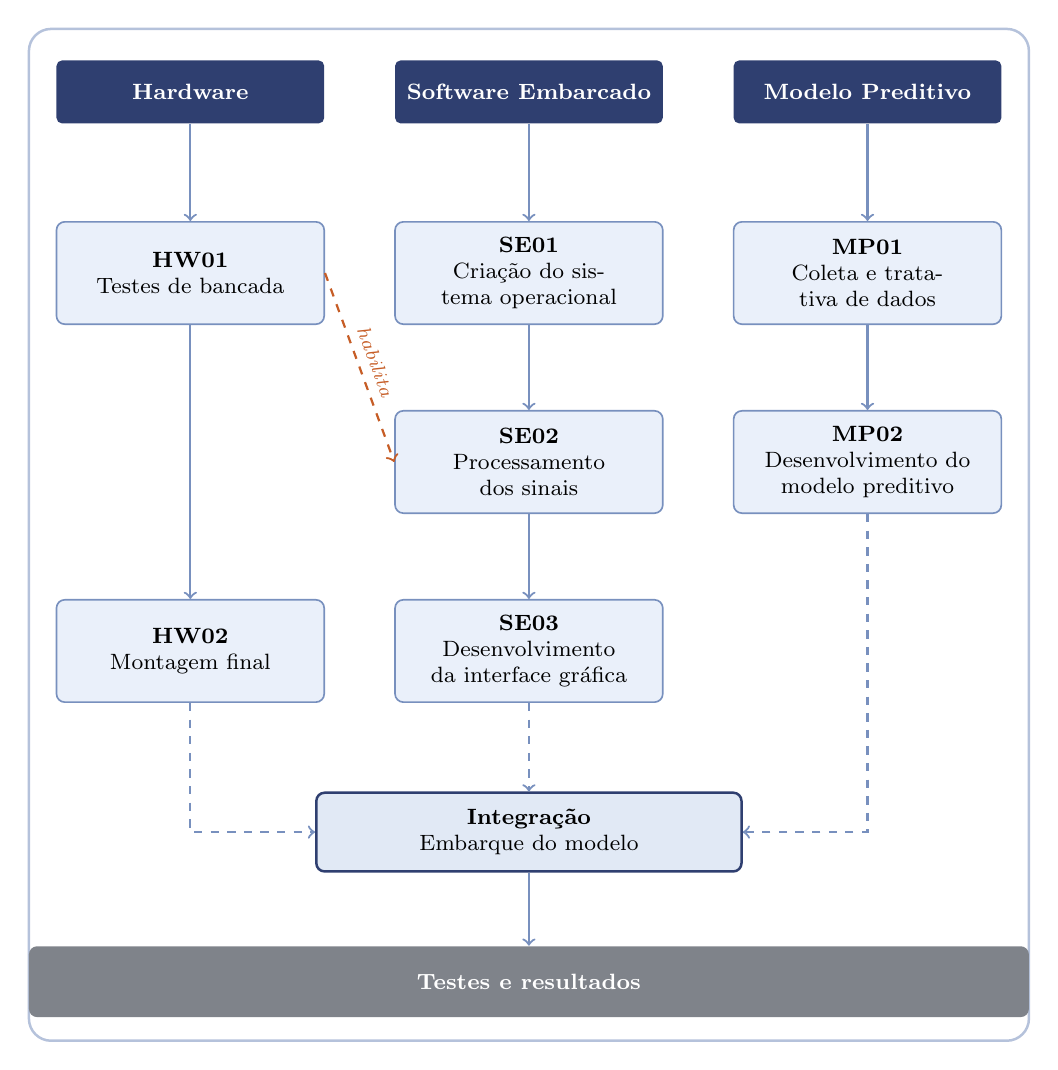
\begin{tikzpicture}[
		font=\footnotesize,
		header/.style={rectangle, rounded corners=2pt, fill=flowhead, text=white,
			font=\footnotesize\bfseries, align=center,
			minimum width=3.4cm, minimum height=0.8cm},
		fstep/.style={rectangle, rounded corners=3pt, draw=flowborder, line width=0.6pt,
			fill=flowbox, align=center, text width=3.0cm,
			minimum width=3.4cm, minimum height=1.3cm, inner sep=3pt},
		fint/.style={rectangle, rounded corners=3pt, draw=flowhead, line width=0.9pt,
			fill=flowint, align=center, text width=5.0cm,
			minimum width=5.4cm, minimum height=1.0cm, inner sep=4pt},
		bar/.style={rectangle, rounded corners=3pt, fill=flowbar, text=white,
			font=\footnotesize\bfseries, align=center, minimum height=0.9cm},
		seq/.style={->, thick, draw=flowborder},
		conv/.style={->, thick, draw=flowborder, dashed},
		xdep/.style={->, thick, draw=flowcross, dashed}
	]
		\draw[rounded corners=8pt, draw=flowborder!55, line width=0.9pt]
			(-2.05,0.8) rectangle (10.65,-12.05);
		% cabeçalhos
		\node[header] (hHW) at (0,0) {Hardware};
		\node[header] (hSE) at (4.3,0) {Software Embarcado};
		\node[header] (hMP) at (8.6,0) {Modelo Preditivo};
		% linha 1
		\node[fstep] (HW01) at (0,-2.3) {\textbf{HW01}\\Testes de bancada};
		\node[fstep] (SE01) at (4.3,-2.3) {\textbf{SE01}\\Criação do sistema operacional};
		\node[fstep] (MP01) at (8.6,-2.3) {\textbf{MP01}\\Coleta e tratativa de dados};
		% linha 2
		\node[fstep] (SE02) at (4.3,-4.7) {\textbf{SE02}\\Processamento dos sinais};
		\node[fstep] (MP02) at (8.6,-4.7) {\textbf{MP02}\\Desenvolvimento do modelo preditivo};
		% linha 3
		\node[fstep] (HW02) at (0,-7.1) {\textbf{HW02}\\Montagem final};
		\node[fstep] (SE03) at (4.3,-7.1) {\textbf{SE03}\\Desenvolvimento da interface gráfica};
		% integração + barra final
		\node[fint] (INT) at (4.3,-9.4) {\textbf{Integração}\\Embarque do modelo};
		\node[bar, minimum width=12.7cm, text width=12.3cm] (TST) at (4.3,-11.3) {Testes e resultados};
		% cabeçalho -> primeira etapa
		\draw[seq] (hHW) -- (HW01);
		\draw[seq] (hSE) -- (SE01);
		\draw[seq] (hMP) -- (MP01);
		% sequência dentro das trilhas
		\draw[seq] (HW01) -- (HW02);
		\draw[seq] (SE01) -- (SE02);
		\draw[seq] (SE02) -- (SE03);
		\draw[seq] (MP01) -- (MP02);
		% dependência entre trilhas: bancada habilita os drivers
		\draw[xdep] (HW01.east) -- node[pos=0.5, sloped, above, font=\scriptsize\itshape, text=flowcross]{habilita} (SE02.west);
		% convergência para a Integração
		\draw[conv] (HW02.south) |- (INT.west);
		\draw[conv] (SE03) -- (INT);
		\draw[conv] (MP02.south) |- (INT.east);
		% integração -> testes
		\draw[seq] (INT) -- (TST);
	\end{tikzpicture}\\
	\textbf{\footnotesize Fonte: Elaborado pelos autores.}
\end{figure}

\textbf{Etapa HW01:} a etapa de testes de bancada consistiu na validação individual de cada componente diretamente sobre a Raspberry Pi 3B+, antes da integração física do dispositivo. Cada sensor foi conectado isoladamente à placa por meio de uma protoboard, o que permitiu verificar a comunicação, a integridade dos sinais e o comportamento elétrico sem a complexidade da montagem completa. O MAX30102 foi validado pelo barramento I\textsuperscript{2}C, confirmando-se o endereçamento do dispositivo e a aquisição do sinal PPG bruto; o DS18B20 foi verificado pelo barramento 1-Wire, incluindo a checagem do resistor de \textit{pull-up} exigido pelo protocolo; os periféricos de alerta, \textit{buzzer} e LED RGB, foram testados via GPIO, e o \textit{display}, pelas interfaces de vídeo e toque. Para cada teste foram desenvolvidos programas em C++ que exercitaram a leitura e o controle dos componentes; esses programas validaram os \textit{drivers} de comunicação e foram posteriormente reaproveitados como base do processo principal da aplicação, desenvolvido em C++ com o \textit{framework} Qt. Essa abordagem incremental de \textit{bring-up} reduziu o risco da etapa de integração, isolando problemas de comunicação ou de configuração ainda na bancada.

\textbf{Etapa HW02:} validados os componentes individualmente, realizou-se a montagem final do protótipo, consolidando a fiação e fixando os elementos no invólucro impresso em PETG. As ligações provisórias de bancada foram substituídas por conexões definitivas e organizadas, reduzindo a probabilidade de mau contato durante a operação contínua. A alimentação partiu de uma fonte chaveada de 5 V conectada a um barramento de distribuição, a partir do qual a Raspberry Pi, o \textit{display} e os ventiladores foram alimentados em paralelo, evitando que toda a corrente trafegasse pela placa de processamento; os sensores e os periféricos de alerta, de baixo consumo, foram alimentados diretamente pelos pinos da Raspberry Pi. Para a gestão térmica, exigida pela operação contínua sob carga de inferência, foram previstos quatro ventiladores: dois de pequeno porte dedicados ao processador e dois maiores para o fluxo de ar interno do invólucro. A fonte foi dimensionada para o consumo agregado desses elementos. O resultado é o dispositivo integrado, fisicamente fechado e pronto para a execução conjunta do \textit{software} embarcado e do modelo preditivo.

\textbf{Etapa SE01:} a primeira etapa do \textit{software} embarcado consistiu na construção da imagem do sistema operacional sobre a qual a aplicação é executada, gerada com o Buildroot a partir da configuração base da Raspberry Pi 3B+. O Buildroot foi adotado por produzir, a partir de uma \textit{toolchain} de compilação cruzada, uma imagem Linux enxuta e reprodutível, com controle fino sobre os pacotes incluídos, característica alinhada às restrições de recursos e aos requisitos de confiabilidade de um dispositivo de uso clínico.

A configuração do \textit{kernel} habilitou, por meio de \textit{device tree overlays}, as interfaces exigidas pelos sensores, I\textsuperscript{2}C para o MAX30102 e 1-Wire para o DS18B20, além da saída de vídeo e da entrada por toque do \textit{display}. Sobre uma base mínima de sistema provida pelo BusyBox, a imagem incorporou os pacotes efetivamente necessários à aplicação: o \textit{runtime} da linguagem C++ e as bibliotecas do \textit{framework} Qt para a interface gráfica, os módulos de \textit{kernel} de comunicação (\texttt{i2c-dev}, \texttt{w1-gpio} e \texttt{w1-therm}) e as dependências de execução do modelo preditivo. A seleção foi mantida em um \textit{defconfig} versionado, garantindo a reprodutibilidade do ambiente e reduzindo o tempo de inicialização e a superfície de falhas do sistema.

\textbf{Etapa SE02:} esta etapa abrangeu o \textit{software} responsável pela leitura dos sensores, pelo processamento dos sinais fisiológicos e pelo cálculo do escore NEWS2. A leitura do MAX30102 foi feita pela interface \textit{/dev/i2c} e a do DS18B20, sensor de temperatura corporal, pelo \textit{driver} \textit{w1-therm}, ambos expostos nativamente pelo \textit{kernel} Linux. A partir do sinal PPG, a frequência cardíaca (FC) e a saturação de oxigênio (SpO\textsubscript{2}) foram extraídas de forma direta, respectivamente pela detecção de picos no componente pulsátil e pela razão de absorção entre os comprimentos de onda vermelho e infravermelho \cite{allen2007photoplethysmography}, enquanto a frequência respiratória (FR) foi estimada a partir das modulações respiratórias do sinal \cite{charlton2018breathing}.

A pressão arterial (PA) é o parâmetro de obtenção não invasiva mais complexa a partir do sinal PPG. Por isso, adotou-se a abordagem mais direta e clinicamente confiável: o registro manual do valor pela equipe de enfermagem por meio da interface do equipamento. Como a pressão arterial é empregada de forma intermitente no NEWS2, essa estratégia atende ao protocolo sem depender de estimativas de menor acurácia.

Os cinco parâmetros foram amostrados em janelas de 30 segundos e, ao fim de cada janela, submetidos ao cálculo do NEWS2 conforme as faixas clínicas do protocolo \cite{smith2013news}. O escore resultante alimentou tanto a classificação imediata de risco quanto o modelo preditivo descrito adiante.

\textbf{Etapa SE03:} a etapa de desenvolvimento da interface gráfica construiu, com o \textit{framework} Qt, a camada de interação entre o sistema e a equipe de saúde, exibida no \textit{display} de toque capacitivo acoplado à plataforma. A renderização foi desacoplada da aquisição e do processamento dos sinais, executados em \textit{threads} distintas, de modo a preservar a responsividade da interface mesmo durante o processamento contínuo.

A tela foi organizada em duas regiões. A primeira apresenta os cinco sinais vitais que compõem o NEWS2, cada um com seu valor, unidade e a cor correspondente à faixa de pontuação do protocolo, facilitando identificar qual parâmetro está alterado. A segunda concentra os dois principais indicadores: o escore NEWS2 atual, com sua classificação de risco (baixo, médio ou alto), e o NEWS2 estimado para um horizonte futuro pelo modelo preditivo, que indica a tendência de evolução do paciente e auxilia a equipe a antecipar intervenções. Como elementos auxiliares, a interface contempla a identificação do paciente, o registro temporal da última atualização e indicadores do estado dos sensores, sinalizando eventuais perdas de contato ou falhas de leitura que possam comprometer a confiabilidade dos dados exibidos.

\textbf{Etapa MP01:} para o desenvolvimento e a validação dos modelos preditivos, foi utilizado o conjunto de dados disponibilizado em \cite{REYNA}. A escolha desse conjunto justifica-se por quatro fatores: (i) sua disponibilidade pública, sem necessidade de processo de credenciamento individual, o que favorece a reprodutibilidade do trabalho; (ii) o volume amostral de 40.336 pacientes, suficiente para o treinamento robusto de modelos com alta capacidade representacional; (iii) a presença de séries temporais com periodicidade horária, contendo as variáveis fisiológicas necessárias ao cálculo do NEWS2; e (iv) o caráter multicêntrico, com dados provenientes de dois sistemas hospitalares distintos (Beth Israel Deaconess Medical Center e Emory University Hospital), o que viabiliza estratégias de validação externa.
Cada registro do conjunto corresponde a uma hora de internação de um paciente, e contempla as variáveis fisiológicas FC, SpO\textsubscript{2}, temperatura, pressão arterial sistólica (PAS), pressão arterial diastólica (PAD), pressão arterial média (PAM) e FR, além de exames laboratoriais e dados demográficos.

A variável-alvo dos modelos preditivos é o valor do NEWS2, calculado conforme as faixas e pesos definidos pelo Royal College of Physicians (2017). Para cada registro horário do conjunto de dados, o escore foi computado a partir das colunas FC, SpO\textsubscript{2}, temperatura, PAS e FR, atribuindo-se a cada variável uma pontuação entre 0 e 3 conforme suas faixas fisiológicas, e somando-se as pontuações parciais para obtenção do escore agregado, que varia de 0 a 20.

O conjunto de dados é processado em quatro etapas sequenciais. Primeiramente, realiza-se a filtragem de pacientes, excluindo-se aqueles com menos de $W + h$ horas de registro, uma vez que estes não comportam a montagem da janela mínima de entrada nem a definição da variável-alvo no horizonte considerado. Em seguida, aplica-se a imputação de valores ausentes por meio da técnica \textit{forward-fill} limitada a uma janela de 4 horas, considerando que medições mais antigas perdem representatividade fisiológica. Para cada valor imputado, uma variável binária adicional é criada de forma a sinalizar a imputação ao modelo, preservando a informação implícita contida no padrão de medição --- informação clinicamente relevante, dado que a frequência de aferição é em si um indicador de instabilidade percebida pela equipe assistencial.

Na terceira etapa, são extraídas estatísticas descritivas para cada variável fisiológica dentro da janela $X_{t-W+1:t}$, incluindo média, desvio padrão, valor mínimo, valor máximo, último valor observado e coeficiente angular do ajuste linear sobre a janela. Adiciona-se ainda o valor do NEWS2 calculado para cada um dos $W$ instantes da janela, dado que sua trajetória histórica constitui uma das características mais informativas para a predição, conforme demonstrado por \citeonline{salehinejad}. Por fim, todas as variáveis numéricas são normalizadas por padronização \textit{z-score} utilizando estatísticas estimadas exclusivamente sobre o conjunto de treinamento, de modo a evitar vazamento de informação.

\textbf{Etapa MP02:} são avaliados três modelos com vieses indutivos distintos, selecionados de modo a cobrir um espectro de complexidade e a permitir comparações metodologicamente significativas. A regressão logística, com regularização $L_{2}$, atua como modelo de referência (\textit{baseline}) e como análogo computacional ao próprio NEWS2. O segundo modelo é o XGBoost, um algoritmo de \textit{gradient boosting} sobre árvores de decisão amplamente consagrado em tarefas tabulares com séries temporais clínicas \cite{churpek2016}. Por fim, emprega-se uma rede neural recorrente do tipo LSTM (\textit{Long Short-Term Memory}), aplicada diretamente sobre a sequência de sinais vitais reamostrados. %*possivelmente desconsiderar XgBoost, que é decisão binária.%

A justificativa metodológica para a comparação desses três modelos reside na cobertura de paradigmas indutivos distintos: linear interpretável, \textit{ensemble} de árvores e rede neural sequencial. Essa escolha permite isolar a contribuição de cada classe de viés indutivo para o desempenho preditivo, ao invés de comparar modelos da mesma família, evitando que os resultados reflitam apenas variações de hiperparâmetros dentro de um único paradigma.




